
\documentclass{article}
\usepackage{amsmath}
\usepackage{listings}
\usepackage{graphicx}
\usepackage[margin=1in]{geometry}
\pagenumbering{gobble}
\setlength{\tabcolsep}{10pt}
\renewcommand{\arraystretch}{1.7}
 
\begin{document}

\section*{\hfil D. Hari Gajian\hfil}

% \begin{center}
% \begin{tabular}{ |cc| } 
%  \hline
%  Time Limit & 2 detik \\
%  \hline 
%  Memory Limit & 256 MB \\
%  \hline
% \end{tabular}
% \end{center}

\subsection*{Deskripsi}

\par\noindent Bocan bekerja di PT. Humble dengan $N$ buah karyawan. Para karyawan dinomori dari $0$ sampai $N-1$. Perusahaan Bocan unik, karena semua karyawannya rendah hati, sampai-sampai seorang bos tidak mau gajinya lebih banyak dari gaji anak buahnya.

\par\noindent Di bulan Februari ini, PT. Humble mendapat keuntungan $X$ gold, mata uang setempat. Keuntungan ini dibagi sepenuhnya pada seluruh karyawan di PT. Humble. Tentukan berapa kemungkinan pembagian gaji yang mungkin. Dua pembagian gaji dikatakan berbeda jika setidaknya ada satu orang yang mendapat gaji berbeda.

\par\noindent Mata uang gold berupa bilangan bulat dan tidak mengenal pecahan, sehingga $X$ beserta pembagiannya berupa bilangan bulat.

\subsection*{Format Masukan}

\par\noindent Baris pertama berisi bilangan $N$ dan $X$.
\par\noindent $N-1$ baris berikutnya masing-masing terdiri dari sebuah bilangan bulat, yang mana baris ke-$i$ menyatakan $p_{i}$, yaitu bos dari karyawan ke-$(i)$. Bos besar perusahaan PT. Humble dianggap sebagai karyawan nomor $0$.

\subsection*{Format Keluaran}

\par\noindent Satu baris berisi jumlah kemungkinan pembagian gaji yang mungkin, dimodulo $10^9+7$.

\subsection*{Contoh Masukan}

\begin{lstlisting}
3 3
0
0
\end{lstlisting}

\subsection*{Contoh Keluaran}

\begin{lstlisting}
5
\end{lstlisting}

\subsection*{Batasan}

\begin{itemize}
  \item $1 \leq N, X \leq 5.000$
  \item $0 \leq p_{i} < i$, untuk $1 \leq i < N$
\end{itemize}

\subsection*{Penjelasan}

\par\noindent Semua kemungkinan pembagian gaji yang mungkin:

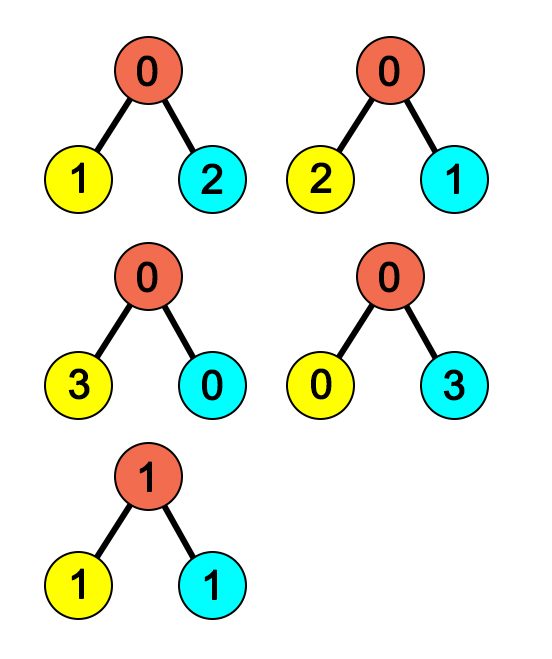
\includegraphics[width=10cm]{sample-1}

\end{document}
